
\begin{frame}
 \frametitle{Main Questions}

What condition or conditions should

\begin{columns}[t]
  \column[T]{5cm}
  \begin{itemize}
    \item the position vector
    \item the coordinates
  \end{itemize}

of a point satisfy\\
for the point to be\\
on a specific\\

\begin{itemize}
    \item line $L$
    \item plane $\mathcal{P}$?
\end{itemize}
  \column[T]{7cm}
    \begin{figure}
        \psfrag{O}{$O$}
        \psfrag{x}{$x$}
        \psfrag{y}{$y$}
        \psfrag{z}{$z$}
        \psfrag{L}{$L$}
        \psfrag{Pi}{$\mathcal{P}$}
        \psfrag{P}{$P(x,y,z)$}
        \psfrag{Q}{$Q(x,y,z)$}
        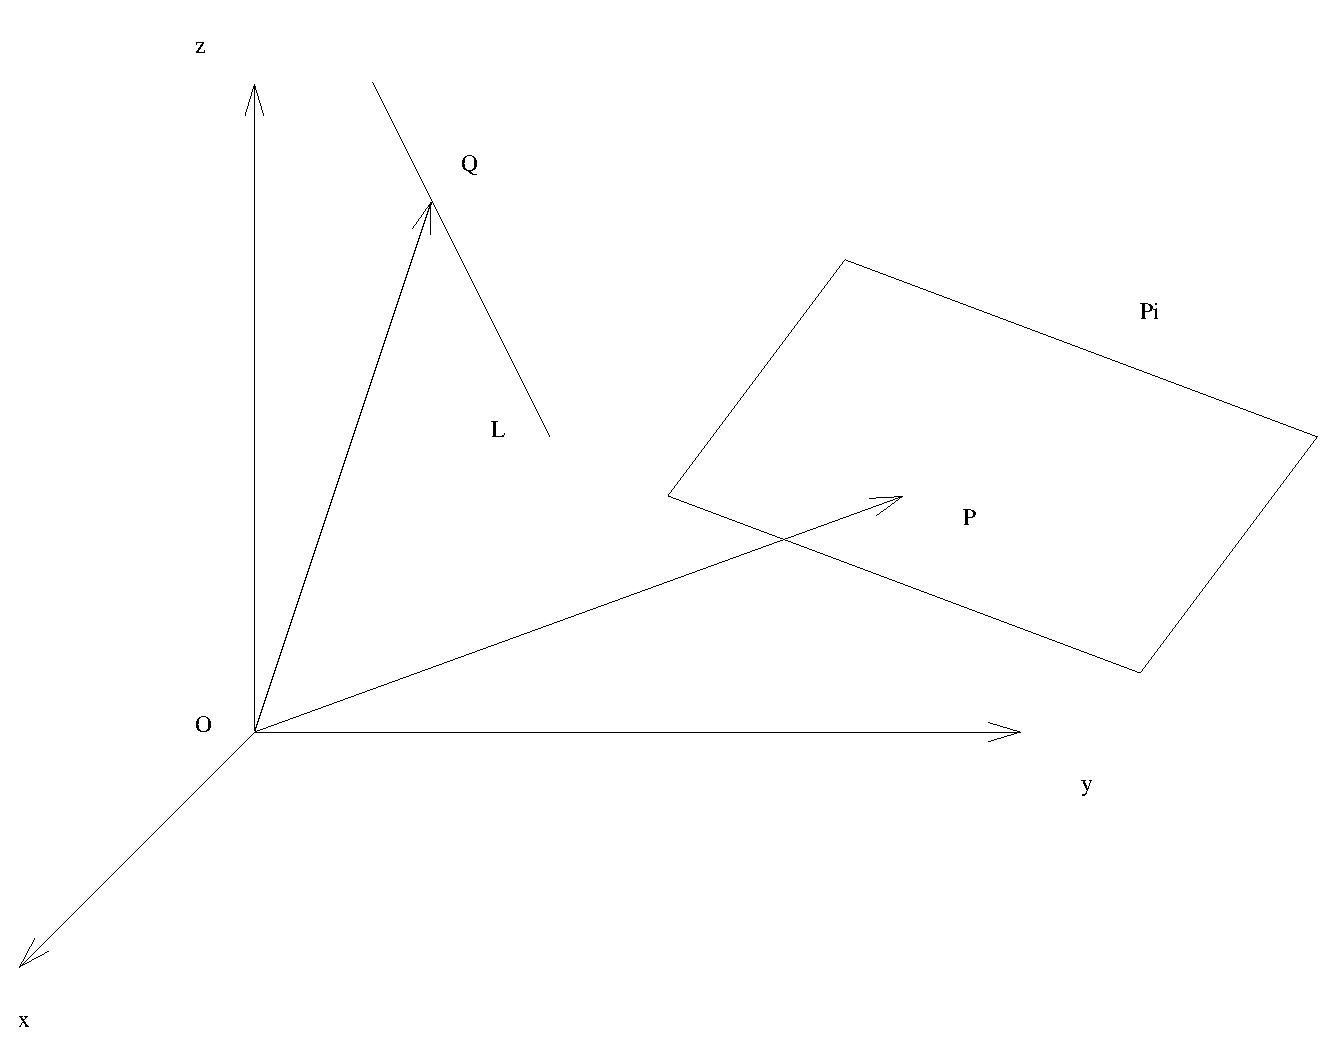
\includegraphics[height=2in]{../images/ok-lines_planes.eps}
    \end{figure}
\end{columns}

Condition(s) in terms of:
\begin{itemize}
    \item position vector $\Rightarrow$ vectorial equations;
    \item coordinates $\Rightarrow$ scalar equations.
\end{itemize}
\end{frame}


\begin{frame}
 \frametitle{Line from Point and Direction}
\begin{columns}
  \column{6cm}
\begin{itemize}
 \item Point $P_0$, with position vector $\textbf{r}_0$;
\item Direction $\leftrightarrow$ non-zero vector $\textbf{u}$.
\end{itemize}
  \column{5cm}
 $L$: line with direction $\textbf{u}$, \\passing through $P_0$
\end{columns}

\bigskip

\begin{columns}
  \column{6cm}
    \uncover<2->{$P$ with position vector $\textbf{r}$ is on $L$ $\leftrightarrow$ \\ }
    \uncover<3->{\medskip $\textbf{P}_0\textbf{P}$ has the same direction as $\textbf{u}$ $\leftrightarrow$\\}
    \uncover<4->{\medskip $\textbf{P}_0\textbf{P}$ is a scalar multiple of $\textbf{u}$ $\leftrightarrow$\\}
    \uncover<5->{\medskip $\textbf{r}-\textbf{r}_0 = t\textbf{u}$  for some real number $t$ }
  \column{6cm}
    \begin{figure}
        \psfrag{O}{$O$}
        \psfrag{x}{$x$}
        \psfrag{y}{$y$}
        \psfrag{z}{$z$}
        \psfrag{L}{$L$}
        \psfrag{P}{$P$}
        \psfrag{P0}{$P_0$}
        \psfrag{r}{$\textbf{r}$}
        \psfrag{u}{$\textbf{u}$}
        \psfrag{r0}{$\textbf{r}_0$}
        \includegraphics[height=1in]{../images/ok-line_point_direction_vector.eps}
    \end{figure}
\end{columns}


\uncover<6->{\bigskip
$$\text{\textcolor[rgb]{0.98,0.00,0.00}{Parametric vectorial equation}: } \quad \boxed{ \textbf{r} = \textbf{r}_0+t\textbf{u} } \quad \text{ for some real number }t$$}

\end{frame}

\begin{frame}
   \frametitle{Line from Point and Direction}
\begin{columns}
  \column{6cm}
\begin{itemize}
 \item Point $P_0(x_0,y_0,z_0)$, $\textbf{r}_0=\langle x_0,y_0,z_0\rangle$;
\item Direction $\textbf{u}=\langle u_1,u_2,u_3\rangle$.
\end{itemize}
  \column{5cm}
 $L$: line with direction $\textbf{u}$, \\passing through $P_0$
\end{columns}

\begin{columns}
  \column{6cm}
    \uncover<2->{$P$ with position vector $\textbf{r}$ is on $L$ $\leftrightarrow$ \\ }
    \uncover<3->{\medskip $\textbf{r} = \textbf{r}_0+t\textbf{u}$ $\leftrightarrow$\\}
    \uncover<4->{\medskip $\langle x,y,z\rangle = \langle x_0,y_0,z_0\rangle + t\langle u_1,u_2,u_3\rangle$ $\leftrightarrow$\\}
    \uncover<5->{\medskip \textcolor[rgb]{0.98,0.00,0.00}{Parametric scalar equations}:\\
    $\boxed{\left\{ \begin{array}{ll}
           x & = x_0 + t u_1 \\
	   y & = y_0 + t u_2 \\
           z & = z_0 + t u_3
          \end{array}
\right.}$  \\ for some real parameter $t$ }

  \column{6.5cm}
    \begin{figure}
        \psfrag{O}{$O$}
        \psfrag{x}{$x$}
        \psfrag{y}{$y$}
        \psfrag{z}{$z$}
        \psfrag{L}{$L$}
        \psfrag{P}{$P(x,y,z)$}
        \psfrag{P0}{$P_0(x_0,y_0,z_0)$}
        \psfrag{r}{$\textbf{r}$}
        \psfrag{u}{$\textbf{u}=\langle u_1,u_2,u_3\rangle$}
        \psfrag{r0}{$\textbf{r}_0$}
        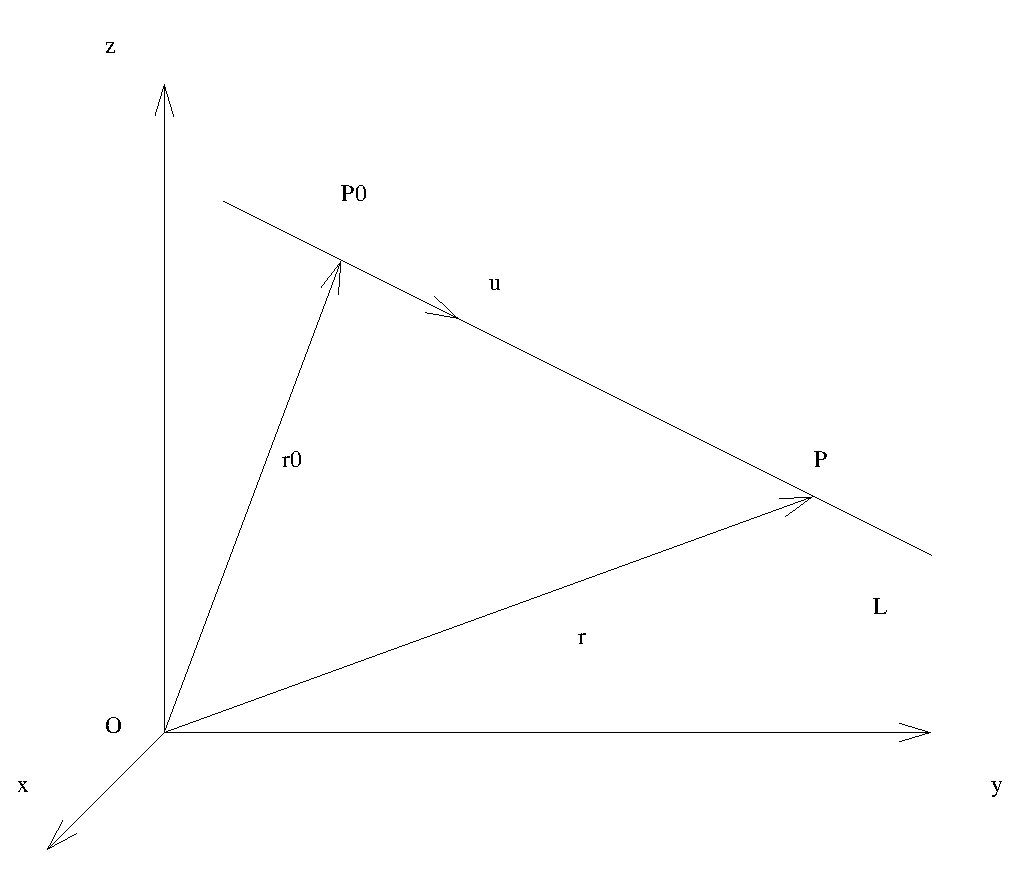
\includegraphics[height=2in]{../images/ok-line_point_direction_scalar.eps}
    \end{figure}
\end{columns}
\end{frame}


\begin{frame}
\uncover<1->{ $$\left\{ \begin{array}{ll}
           x & = x_0 + t u_1 \\
	   y & = y_0 + t u_2 \\
           z & = z_0 + t u_3
          \end{array}
\right. \Longrightarrow \boxed{\frac{x-x_0}{u_1} = \frac{y-y_0}{u_2} = \frac{z-z_0}{u_3}} \text{ \textcolor[rgb]{0.98,0.00,0.00}{Symmetric equations}}$$}

\uncover<2->{Caution! If $u_2=0$ (for example), then:
%
$$\frac{x-x_0}{u_1} = \frac{z-z_0}{u_3} \quad  \text{ and } \quad y=y_0 $$}

\uncover<3->{Example: Line with direction $\textbf{u} = \langle 4,5,6\rangle$ through $P_0(1,2,3)$:}
\begin{itemize}
 \item<4-> Parametric vectorial equation:
%
$$\textbf{r} = \langle 1,2,3\rangle + t \langle 4,5,6\rangle \leftrightarrow
\textbf{r} = \langle 1+4t, 2+5t, 3+6t\rangle$$
%
\item<5-> Parametric scalar equations:
%
$$\left\{ \begin{array}{ll}
           x & = 1 + 4t \\
	   y & = 2+5t \\
           z & = 3+6t
          \end{array}
\right. , \quad t \text{ real number.}$$
%
\item<6-> Symmetric equations:
%
$$\frac{x-1}{4} = \frac{y-2}{5} = \frac{z-3}{6}\; .$$
\end{itemize}

\end{frame}

\begin{frame}
 \frametitle{Line from Two Points}
Given: distinct points $P_0$ and $P_1$, with position vectors $\textbf{r}_0$ and $\textbf{r}_1$. \\

$L$: line through $P_0$ and $P_1$.

\bigskip

\begin{columns}
  \column{6cm}

  \uncover<2->{Direction of $L$: $\textbf{u} = \textbf{r}_1 - \textbf{r}_0$.\\}
  \uncover<5->{$\textbf{u} = \langle x_1-x_0,y_1-y_0,z_1-z_0\rangle$}

  \uncover<3->{\medskip \textcolor[rgb]{0.98,0.00,0.00}{Parametric vectorial equation} of $L$:\\
  $\textbf{r} = \textbf{r}_0 + t(\textbf{r}_1-\textbf{r}_0)$\\}

  \uncover<4->{\medskip Equivalent equation:\\
  $\textbf{r} = (1-t)\textbf{r}_0 + t\textbf{r}_1$}
  \column{6cm}
    \only<2-4>{\begin{figure}
        \psfrag{O}{$O$}
        \psfrag{L}{$L$}
        \psfrag{P}{$P$}
        \psfrag{P0}{$P_0$}
        \psfrag{P1}{$P_1$}
        \psfrag{r}{$\textbf{r}$}
        \psfrag{u}{$\textbf{u}$}
        \psfrag{r0}{$\textbf{r}_0$}
        \psfrag{r1}{$\textbf{r}_1$}
        \includegraphics[height=1.5in]{../images/ok-line_point_point_vector.eps}
    \end{figure}}
    \only<5->{\begin{figure}
        \psfrag{O}{$O$}
        \psfrag{x}{$x$}
        \psfrag{y}{$y$}
        \psfrag{z}{$z$}
        \psfrag{L}{$L$}
        \psfrag{P}{$P(x,y,z)$}
        \psfrag{P0}{$P_0(x_0,y_0,z_0)$}
        \psfrag{P1}{$P_1(x_1,y_1,z_1)$}
        \psfrag{r}{$\textbf{r}$}
        \psfrag{u}{$\textbf{u}$}
        \psfrag{r0}{$\textbf{r}_0$}
        \psfrag{r1}{$\textbf{r}_1$}
        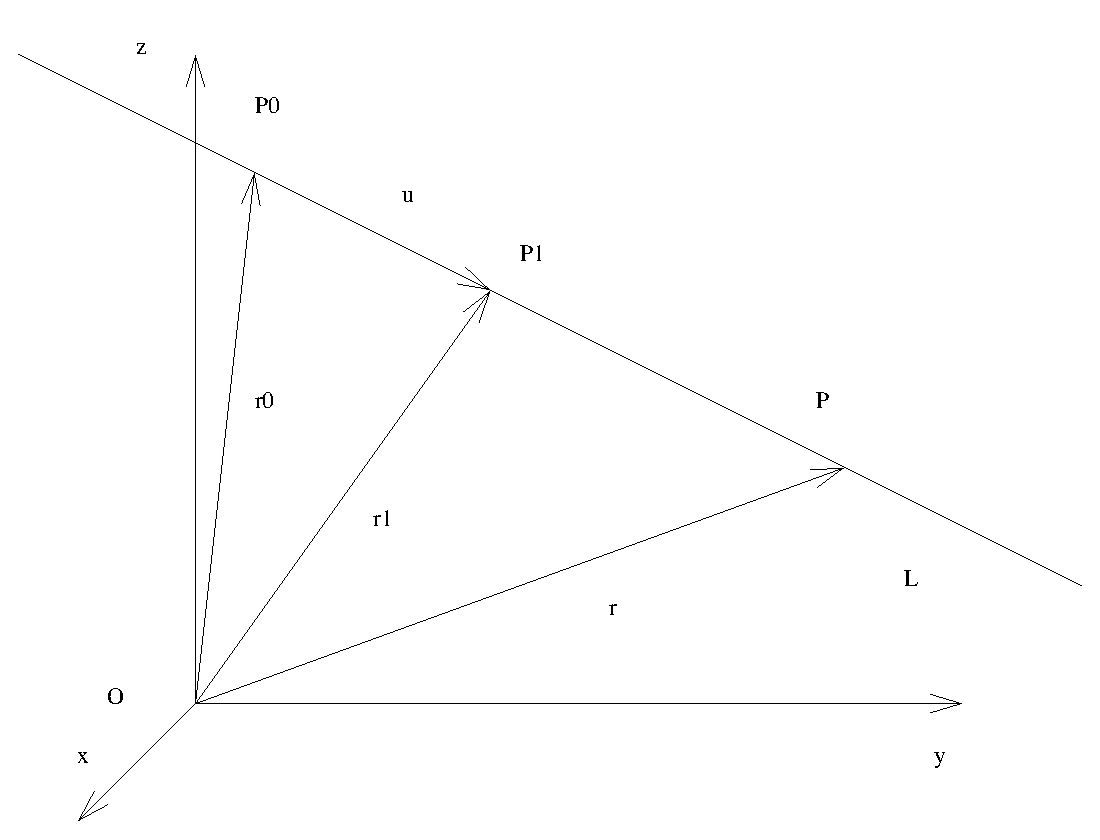
\includegraphics[height=1.5in]{../images/ok-line_point_point_scalar.eps}
    \end{figure}}
\end{columns}

\uncover<5->{\textcolor[rgb]{0.98,0.00,0.00}{Parametric scalar equations}:
%
$$\left\{ \begin{array}{ll}
           x & = x_0 + t(x_1-x_0) \\
	   y & = y_0 + t(y_1-y_0) \\
           z & = z_0 + t(z_1-z_0)
          \end{array}
\right. \leftrightarrow \left\{ \begin{array}{ll}
           x & = (1-t)x_0 + tx_1 \\
	   y & = (1-t)y_0 + ty_1 \\
           z & = (1-t)z_0 + tz_1
          \end{array}
\right. , \quad t \text{ real number.}$$}
\end{frame}


\begin{frame}
 \frametitle{Example}

Line $L$ through $P_0(1,2,3)$ and $P_1(5,2,1)$.

\begin{itemize}
 \item<2-> Direction of $L$: $\textbf{u} = \textbf{r}_1-\textbf{r}_0 = \langle 4, 0, -2\rangle$.
\item<3-> Parametric vectorial equation:
%
$$\textbf{r} = \langle 1,2,3\rangle + t \langle 4, 0 -2\rangle \leftrightarrow \textbf{r} = \langle 1+4t, 2, 3-2t\rangle\; .$$
%
\item<4-> Parametric scalar equations:
$$\left\{ \begin{array}{ll}
           x & = 1+4t \\
	   y & = 2 \\
           z & = 3-2t
          \end{array}
\right. , \quad t \text{ real number.}$$
%
\item<5-> Symmetric equations:
%
$$\frac{x-1}{4} = \frac{z-3}{-2} \quad \text{ and } \quad y=2\; .$$
\end{itemize}

\end{frame}

\begin{frame}
 \frametitle{Plane from Point and Normal}

\begin{columns}
  \column{6cm}
\begin{itemize}
 \item<1-> Point $P_0$, with position vector $\textbf{r}_0$;\\
 \uncover<5->{$\textbf{r}_0 = \langle x_0,y_0,z_0\rangle$}
\item<1-> Direction $\textbf{n}$, non-zero vector.\\
  \uncover<5->{$\textbf{n} = \langle a,b,c\rangle$}
\end{itemize}
  \column{6cm}
$\mathcal{P}$: plane\\
passing through $P_0$ and \\
normal to direction $\textbf{n}$.
\end{columns}

\bigskip

\begin{columns}
  \column{6cm}
\begin{center}
 \uncover<2-4>{A point $P(\textbf{r})$ is on $\mathcal{P}$ $\longleftrightarrow$\\}
 \uncover<5->{A point $P(x,y,z)$ is on $\mathcal{P}$ $\longleftrightarrow$\\}
 \uncover<3-4>{\medskip $\textbf{P}_0\textbf{P}$ is normal to $\textbf{n}$ $\longleftrightarrow$\\}
 \uncover<4->{\medskip \textcolor[rgb]{0.98,0.00,0.00}{Implicit vectorial equation}: \\
 $\boxed{ (\textbf{r}-\textbf{r}_0) \cdot \textbf{n} = 0 \;.}$\\}
 \uncover<6->{\medskip\textcolor[rgb]{0.98,0.00,0.00}{Implicit scalar equation}: \\
 $\langle x-x_0, y-y_0, z-z_0\rangle \cdot \langle a,b,c\rangle = 0$\\
 $\boxed{a(x-x_0) + b(y-y_0)+c(z-z_0) = 0}$}
\end{center}

  \column{6cm}
    \only<2-4>{\begin{figure}
        \psfrag{O}{$O$}
        \psfrag{Pi}{$\mathcal{P}$}
        \psfrag{P}{$P$}
        \psfrag{P0}{$P_0$}
        \psfrag{r}{$\textbf{r}$}
        \psfrag{n}{$\textbf{n}$}
        \psfrag{r0}{$\textbf{r}_0$}
        \includegraphics[height=1.5in]{../images/ok-plane_point_normal_vector.eps}
    \end{figure}}
    \only<5->{\begin{figure}
        \psfrag{O}{$O$}
        \psfrag{x}{$x$}
        \psfrag{y}{$y$}
        \psfrag{z}{$z$}
        \psfrag{Pi}{$\mathcal{P}$}
        \psfrag{P}{$P(x,y,z)$}
        \psfrag{P0}{$P_0(x_0,y_0,z_0)$}
        \psfrag{r}{$\textbf{r}$}
        \psfrag{n}{$\textbf{n}=\langle a,b,c \rangle$}
        \psfrag{r0}{$\textbf{r}_0$}
        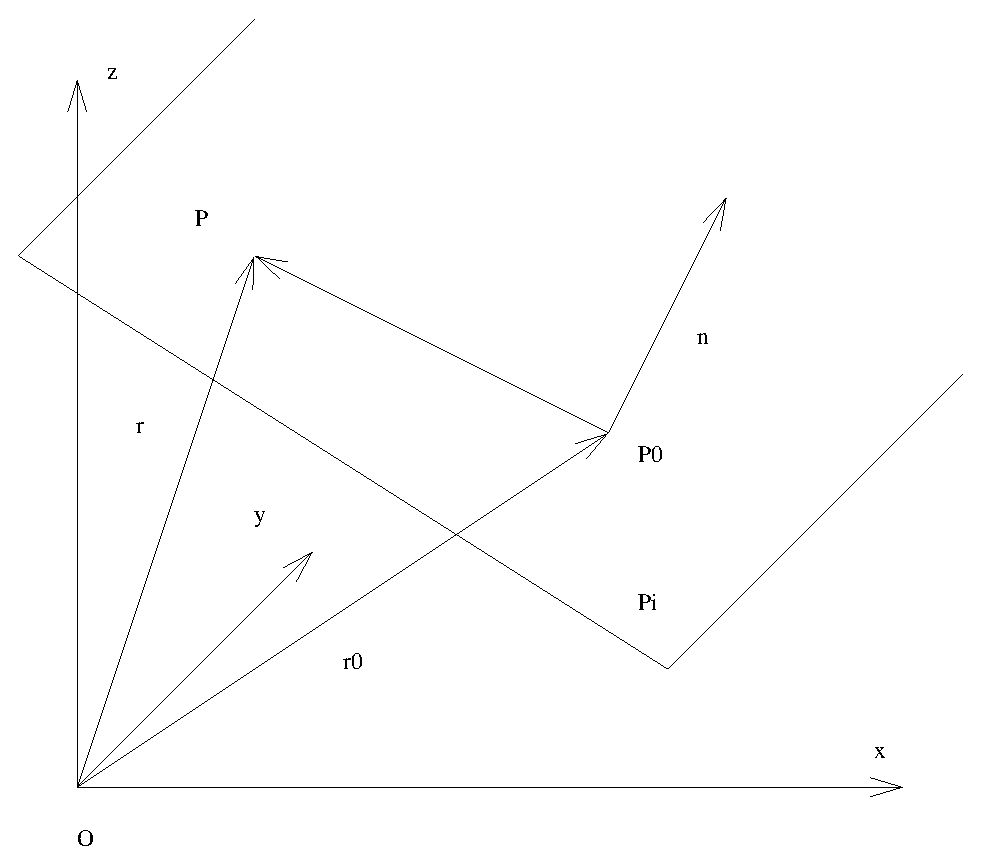
\includegraphics[height=1.5in]{../images/ok-plane_point_normal_scalar.eps}
    \end{figure}}
\end{columns}
\end{frame}

\begin{frame}
 \frametitle{Example}

Equation of the plane
\begin{itemize}
 \item Passing through $P_0(1,2,3)$;
\item Normal to the direction $\textbf{n} = \langle 6,5,4\rangle$:
\end{itemize}
%
\pause
$$6(x-1) + 5(y-2) + 4(z-3) = 0$$
%
$$6x +5y+4z = 28$$

\pause General equation of a plane:
%
$$ax+by+cz = d$$
%
Coefficients $a,b,c$: \pause components of normal to the plane,
%
$$\textbf{n} = \langle a,b,c\rangle\; .$$

\end{frame}

\begin{frame}
 \frametitle{Plane from Point and two Directions}

\begin{columns}
  \column{6cm}
  Point $P_0$, with position vector $\textbf{r}_0$;\\
  Non-parallel directions $\textbf{u}$ and $\textbf{v}$.
  \column{6cm}
    $\mathcal{P}$: plane through $P_0$ and \\
    parallel to both $\textbf{u}$ and $\textbf{v}$.
\end{columns}

\begin{columns}
  \column{5.5cm}
  \only<2>{Normal direction $\textbf{n} = \textbf{u} \times \textbf{v} \neq \textbf{0}$ \\
  \medskip \textcolor[rgb]{0.98,0.00,0.00}{Implicit vectorial equation}:
  $$P(\textbf{r}) \text{ is on } \mathcal{P} \Longleftrightarrow \boxed{(\textbf{r}-\textbf{r}_0) \cdot \textbf{n} = 0}$$
  Interpretation:\\
  $$\text{Vol}(R(\textbf{r} - \textbf{r}_0,\textbf{u},\textbf{v})) = 0$$}
  \only<3>{$P(\textbf{r})$ is on the plane $\mathcal{P}$ $\leftrightarrow$\\
  \medskip
    $\textbf{P}_0\textbf{P}$ is a combination of $\textbf{u}$, $\textbf{v}$
    $\leftrightarrow$\\
    \medskip
    There are scalars $s$, $t$ such that \\
    $\textbf{r}-\textbf{r}_0= s\textbf{u} + t\textbf{v} \leftrightarrow $\\
    \medskip
    \textcolor[rgb]{0.98,0.00,0.00}{Parametric vectorial equation}:
    $$\boxed{ \textbf{r} = \textbf{r}_0 + s\textbf{u} + t\textbf{v} \; }$$
    for some parameters $s$ and $t$}
  \only<4>{
  \textcolor[rgb]{0.98,0.00,0.00}{Parametric vectorial equation}:
  $$\textbf{r} = \textbf{r}_0 + s\textbf{u} + t\textbf{v}$$
  $P_0(x_0,y_0,z_0)$, $P(x,y,z)$\\
  $\textbf{u} = \langle u_1,u_2,u_3\rangle$,
  $\textbf{v}=\langle v_1,v_2,v_3\rangle$\\
  \medskip\textcolor[rgb]{0.98,0.00,0.00}{Parametric scalar equations}:
  $$\left\{ \begin{array}{ll}
           x = & x_0 + su_1+tv_1 \\
	   y = & y_0 + su_2+tv_2 \\
           z = & z_0 + su_3+tv_3
          \end{array}
\right.$$ for  $s$, $t$  real parameters.}
  \column{7cm}
  \only<1>{\begin{figure}
        \psfrag{O}{$O$}
        \psfrag{Pi}{$\mathcal{P}$}
        \psfrag{P}{$P$}
        \psfrag{P0}{$P_0$}
        \psfrag{r}{$\textbf{r}$}
        \psfrag{u}{$\textbf{u}$}
        \psfrag{v}{$\textbf{v}$}
        \psfrag{r0}{$\textbf{r}_0$}
        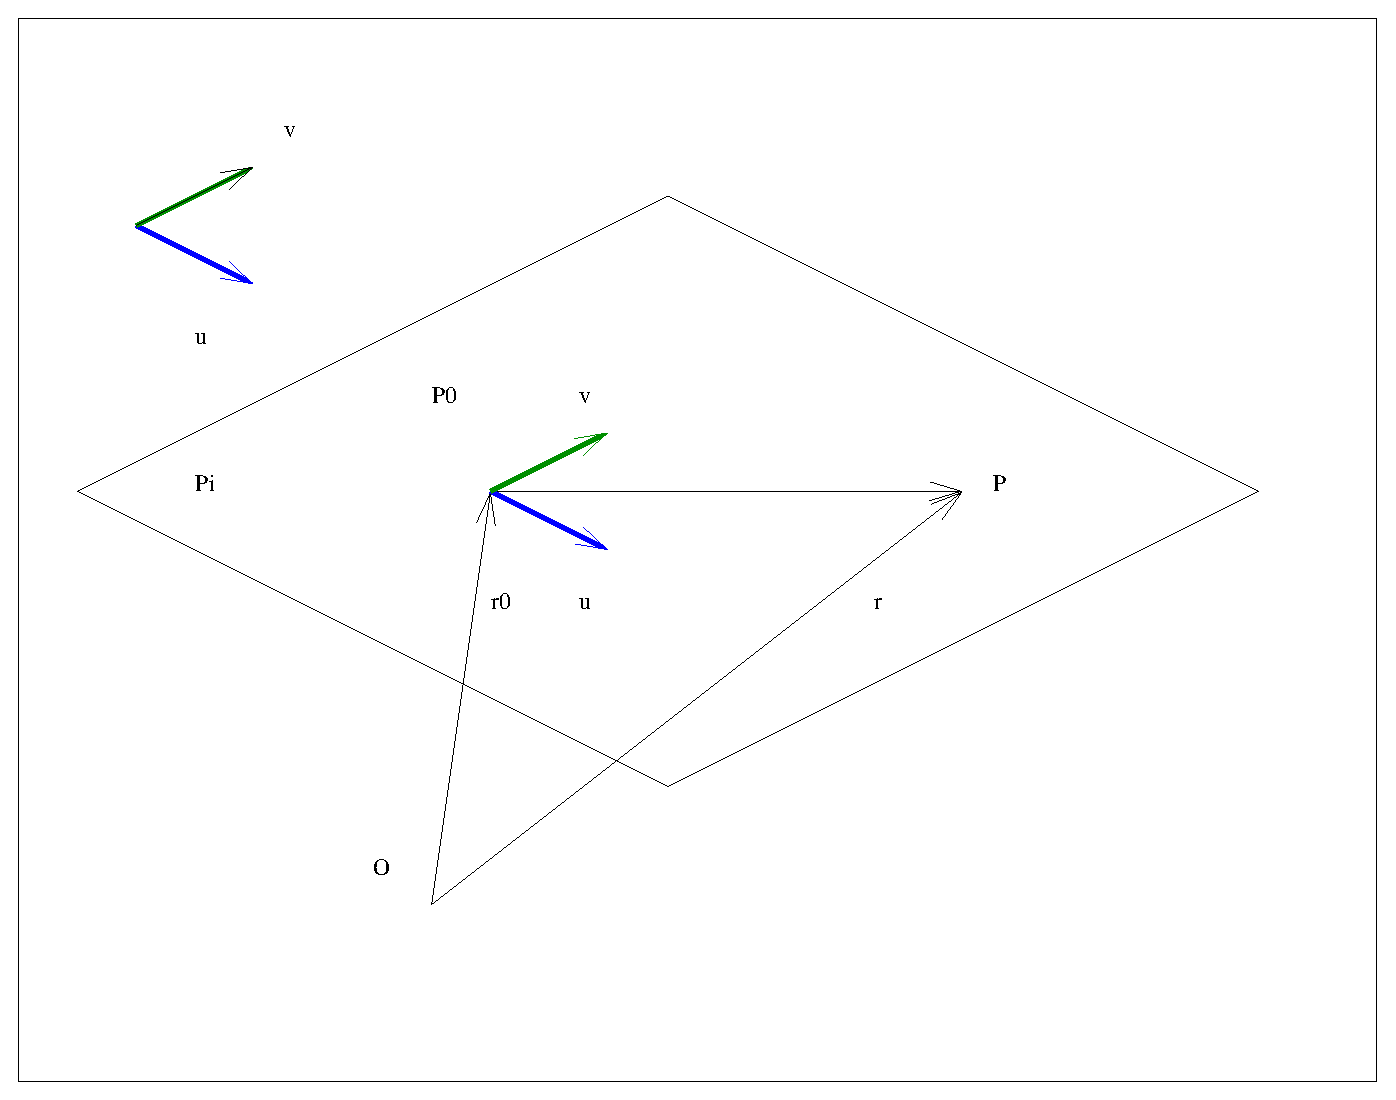
\includegraphics[height=2in]{../images/ok-plane_point_directions.eps}
    \end{figure}}
  \only<2>{\begin{figure}
        \psfrag{O}{$O$}
        \psfrag{Pi}{$\mathcal{P}$}
        \psfrag{P}{$P$}
        \psfrag{P0}{$P_0$}
        \psfrag{r}{$\textbf{r}$}
        \psfrag{n}{$\textbf{n}$}
        \psfrag{u}{$\textbf{u}$}
        \psfrag{v}{$\textbf{v}$}
        \psfrag{r0}{$\textbf{r}_0$}
        \includegraphics[height=2in]{../images/ok-plane_point_directions_vector.eps}
    \end{figure}}
    \only<3>{\begin{figure}
        \psfrag{O}{$O$}
        \psfrag{x}{$x$}
        \psfrag{y}{$y$}
        \psfrag{z}{$z$}
        \psfrag{Pi}{$\mathcal{P}$}
        \psfrag{P}{$P$}
        \psfrag{P0}{$P_0$}
        \psfrag{r}{$\textbf{r}$}
        \psfrag{n}{$\textbf{n}$}
        \psfrag{u}{$\textbf{u}$}
        \psfrag{v}{$\textbf{v}$}
        \psfrag{su}{$s\textbf{u}$}
        \psfrag{tv}{$t\textbf{v}$}
        \psfrag{r0}{$\textbf{r}_0$}
        \includegraphics[height=2in]{../images/ok-plane_point_parametric_vectorial.eps}
    \end{figure}}
  \only<4>{\begin{figure}
        \psfrag{O}{$O$}
        \psfrag{x}{$x$}
        \psfrag{y}{$y$}
        \psfrag{z}{$z$}
        \psfrag{Pi}{$\mathcal{P}$}
        \psfrag{P}{$P$}
        \psfrag{P0}{$P_0$}
        \psfrag{r}{$\textbf{r}$}
        \psfrag{n}{$\textbf{n}$}
        \psfrag{u}{$\textbf{u}$}
        \psfrag{v}{$\textbf{v}$}
        \psfrag{su}{$s\textbf{u}$}
        \psfrag{tv}{$t\textbf{v}$}
        \psfrag{r0}{$\textbf{r}_0$}
        \includegraphics[height=2in]{../images/ok-plane_point_directions_scalar.eps}
    \end{figure}}
\end{columns}
\end{frame}


\begin{frame}
 \frametitle{Example}

$P_0(1,2,3)$, $\textbf{u}=\langle -1,0,2\rangle$, $\textbf{v} = \langle 0,-2,1\rangle$.\pause
%
$$\textbf{n} = \textbf{u} \times \textbf{v} = \left| \begin{array}{ccc}
                           \textbf{i} & \textbf{j} & \textbf{k} \\
			   -1 & 0 & 2 \\
                           0 & -2 & 1
                          \end{array}
\right| = 4\textbf{i}+\textbf{j} +2\textbf{k}$$
%
$$4(x-1)+1(y-2) + 2(z-3) = 0 \Longleftrightarrow 4x+y+2z = 12$$
%
\pause Implicit scalar equation:
%
$$4x+y+2z = 12\; .$$

\pause Parametric vectorial equation:
%
$$\langle x, y, z \rangle = \langle 1,2,3\rangle + s\langle -1, 0, 2\rangle + t\langle 0,-2,1\rangle$$

\pause Parametric scalar equations:
%
$$\left\{ \begin{array}{ll}
           x & = 1 -s \\
           y & = 2-2t \\
           z & = 3 +2s +t
          \end{array}
\right. \quad s,t \text{ real parameters}.$$
%
\end{frame}


\begin{frame}
 \frametitle{Plane from Three Points}

\begin{columns}
  \column{6cm}
  Three non-collinear points\\
   $P_0(\textbf{r}_0)$, $P_1(\textbf{r}_1)$, $P_2(\textbf{r}_2)$
  \column{6cm}
  Plane $\mathcal{P}$\\
   passing through $P_0$, $P_1$, and $P_2$.
\end{columns}

\begin{columns}
  \column{7cm}
  \only<2>{Passing through $P_0(\textbf{r}_0)$\\
  Parallel to \\
  $\textbf{u} = \textbf{P}_0\textbf{P}_1 = \textbf{r}_1 -\textbf{r}_0$\\
    $\textbf{v} = \textbf{P}_0\textbf{P}_2 = \textbf{r}_2-\textbf{r}_0$.\\
Normal $\textbf{n} = \textbf{u} \times \textbf{v} =
(\textbf{r}_1-\textbf{r}_0) \times (\textbf{r}_2-\textbf{r}_0)$  \\

\textcolor[rgb]{0.98,0.00,0.00}{Implicit vectorial equation}:
  $$(\textbf{r}-\textbf{r}_0) \cdot \textbf{n} = 0$$
  %
  $$\boxed{(\textbf{r}-\textbf{r}_0) \cdot [(\textbf{r}_1-\textbf{r}_0) \times (\textbf{r}_2-\textbf{r}_0)] = 0}$$
%
$$\text{Vol}(R(\textbf{P}_0\textbf{P}, \textbf{P}_0\textbf{P}_1, \textbf{P}_0\textbf{P}_2)) = 0$$
  }

 \only<3>{
 \textcolor[rgb]{0.98,0.00,0.00}{Implicit vectorial equation}:
  %
  $$(\textbf{r}-\textbf{r}_0) \cdot [(\textbf{r}_1-\textbf{r}_0) \times (\textbf{r}_2-\textbf{r}_0)] = 0$$

 $P_0(x_0,y_0,z_0)$, $P_1(x_1,y_1,z_1)$, $P_2(x_2,y_2,z_2)$:\\

$P(x,y,z)$ is on plane $\mathcal{P}$:\\
\medskip
\textcolor[rgb]{0.98,0.00,0.00}{Implicit scalar equation}:
%
$$\left| \begin{array}{ccc}
          x-x_0 & y-y_0 & z-z_0 \\
          x_1-x_0 & y_1-y_0 & z_1-z_0 \\
          x_2-x_0 & y_2-y_0 & z_2-z_0	
         \end{array}
\right| = 0\; .$$
%
  }

  \column{5.5cm}
    \begin{figure}
        \psfrag{O}{$O$}
        \psfrag{Pi}{$\mathcal{P}$}
        \psfrag{P}{$P$}
        \psfrag{P0}{$P_0$}
        \psfrag{P1}{$P_1$}
        \psfrag{P2}{$P_2$}
        \psfrag{r}{$\textbf{r}$}
        \psfrag{r0}{$\textbf{r}_0$}
        \psfrag{r1}{$\textbf{r}_1$}
        \psfrag{r2}{$\textbf{r}_2$}
        \psfrag{n}{$\textbf{n}$}
        \psfrag{u}{$\textbf{u}$}
        \psfrag{v}{$\textbf{v}$}
        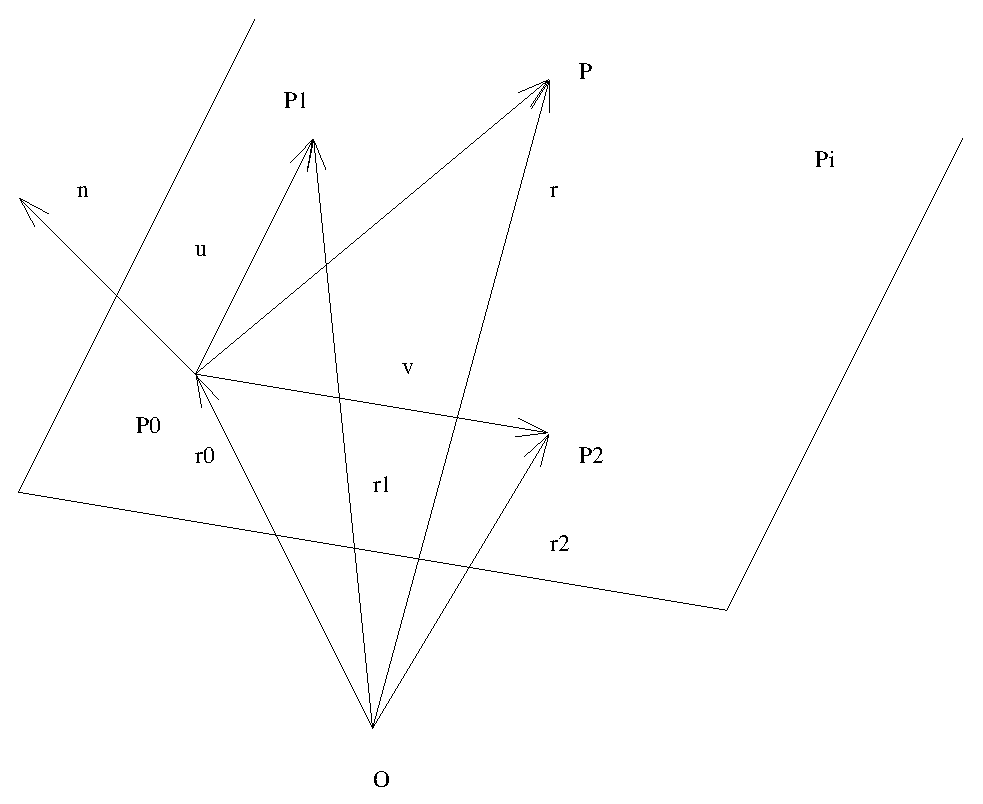
\includegraphics[height=2in]{../images/ok-plane_three_points.eps}
    \end{figure}
\end{columns}

\end{frame}

\begin{frame}
 \frametitle{Example}

$P_0(a,0,0)$, $P_1(0,b,0)$, $P_2(0,0,c)$ distinct points on axes.

$\mathcal{P}$: plane through $P_0$, $P_1$, $P_2$ = plane with given intercepts.

\bigskip

\begin{columns}
  \column{7cm}
  $\mathcal{P}$: parallel to \\
  $\textbf{P}_0\textbf{P}_1 = \langle -a, b, 0\rangle$,
    $\textbf{P}_0\textbf{P}_2 = \langle -a, 0 c\rangle$\\
    Normal to:
$\textbf{n} = \textbf{P}_0\textbf{P}_1 \times \textbf{P}_0\textbf{P}_2$
$$\textbf{n} =
\left| \begin{array}{ccc}
        \textbf{i} & \textbf{j} & \textbf{k} \\
	-a & b & 0 \\
        -a & 0 & c
       \end{array}
 \right| = bc \textbf{i} + ac \textbf{j} + ab \textbf{k}\; .$$
Implicit scalar equation of plane:
%
$$\langle x-a, y, z \rangle \cdot \langle bc, ac, ab \rangle = 0$$
%
$$bcx+acy + abz = abc \Longleftrightarrow \boxed{\frac{x}{a} + \frac{y}{b} + \frac{z}{c} = 1}$$
  \column{5.5cm}
     \begin{figure}
        \psfrag{O}{$O$}
        \psfrag{x}{$x$}
        \psfrag{y}{$y$}
        \psfrag{z}{$z$}
        \psfrag{A}{$P_0(a,0,0)$}
        \psfrag{B}{$P_1(0,b,0)$}
        \psfrag{C}{$P_2(0,0,c)$}
        \psfrag{n}{$\textbf{n}$}
        \psfrag{u}{$\textbf{u}$}
        \psfrag{v}{$\textbf{v}$}
        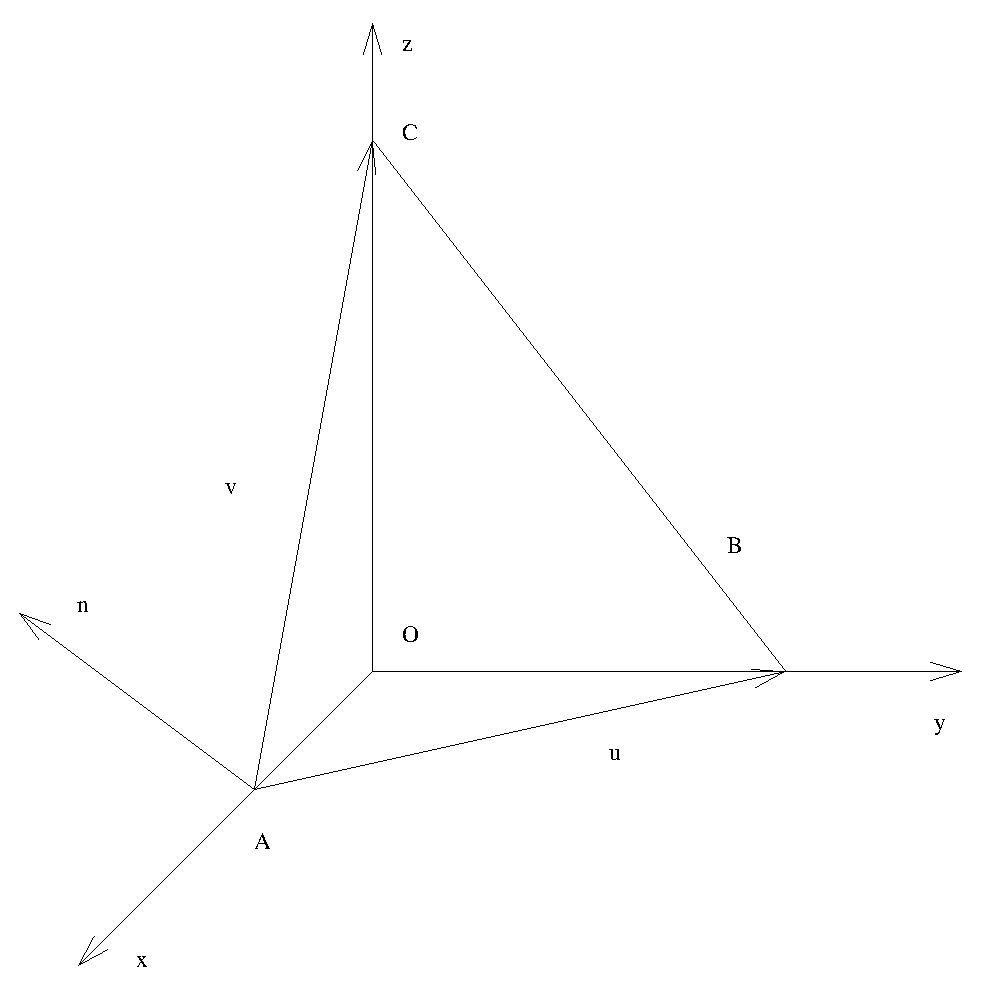
\includegraphics[width=2in]{../images/ok-plane_intercepts.eps}
    \end{figure}
\end{columns}
\end{frame}

\begin{frame}
 \frametitle{Main Questions}

\begin{itemize}
  \item Geometric objects:
  \begin{itemize}
    \item Points: $P(\textbf{r})$.
    \item Lines: $L$: $\textbf{r}= \textbf{r}_0 + t\textbf{u}$
    \item Planes: $\mathcal{P}$: $(\textbf{r}-\textbf{r}_0)\cdot \textbf{n} =0$
  \end{itemize}

  \item Relationships/Geometric Quantities:
  \begin{itemize}
      \item Parallelism
      \item Perpendicularity
      \item Angles
      \item Distances
      \item Intersections
  \end{itemize}
\end{itemize}
\end{frame}

\begin{frame}
  \frametitle{Point and line}
  Point $P(\textbf{r}_1)$ \hspace{2cm} Line $L: \quad \textbf{r}=\textbf{r}_0+t\textbf{u}$

  \begin{columns}
  \column{6cm}
  \textcolor[rgb]{0.98,0.00,0.00}{Distance} from $P$ to $L$:
  \uncover<2->{
  $$d(P,L) = |\textbf{\text{orth}}_{\bm{u}}(\textbf{r}_1-\textbf{r}_0)|$$
  $$\boxed{d(P,L) = \frac{|(\textbf{r}_1-\textbf{r}_0) \times \textbf{u}|}{|\textbf{u}|}}$$}
  %
  \column{6.5cm}
      \begin{figure}
        \psfrag{L}{$L$}
        \psfrag{P}{$P(\textbf{r}_1)$}
        \psfrag{P0}{$P_0(\textbf{r}_0)$}
        \psfrag{u}{$\textbf{u}$}
        \psfrag{r12}{$\textbf{r}_1-\textbf{r}_0$}
        \psfrag{orth}{$\textbf{\text{orth}}_{\bm{u}}(\textbf{r}_1-\textbf{r}_0)$}
        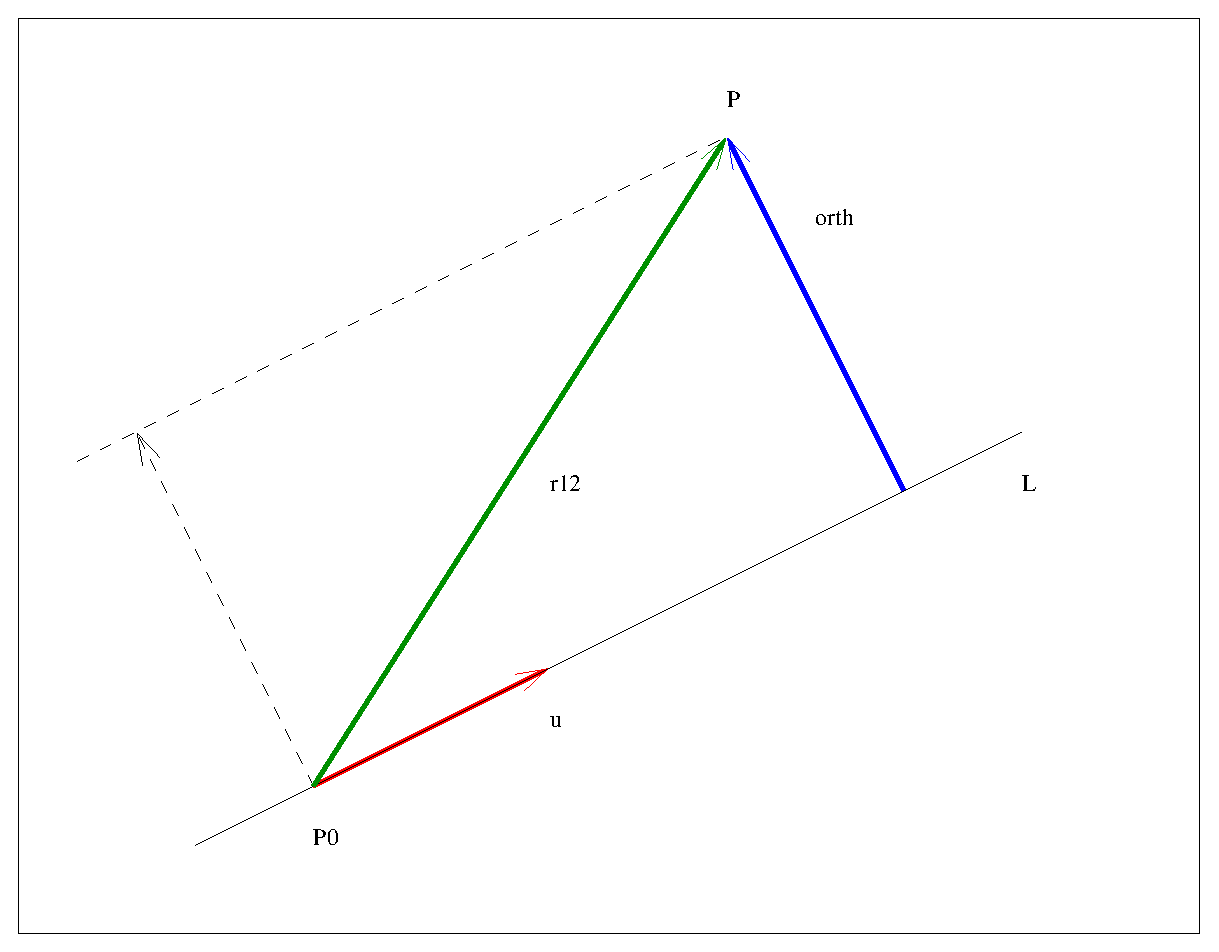
\includegraphics[height=2in]{../images/ok-distance_point_line.eps}
    \end{figure}
    \end{columns}
\end{frame}

\begin{frame}
  \frametitle{Point and plane}
  Point $P(\textbf{r}_1)$ \hspace{2cm} Plane $\mathcal{P}: \quad (\textbf{r}-\textbf{r}_0)\cdot \textbf{n} = 0$
\bigskip
  \begin{columns}
  \column{6cm}
  \textcolor[rgb]{0.98,0.00,0.00}{Distance} from $P$ to $\mathcal{P}$:
  \uncover<2->{
  $$d(P,\mathcal{P}) = |\textbf{\text{proj}}_{\bm{n}}(\textbf{r}_1-\textbf{r}_0)|$$
  $$d(P,\mathcal{P}) = \frac{|(\textbf{r}_1-\textbf{r}_0) \cdot \textbf{n}|}{|\textbf{n}|}$$}
  %
  \uncover<3->{
  \textcolor[rgb]{0.98,0.00,0.00}{Scalar equation}:
  $P(x_1,y_1,z_1)$
   $$\mathcal{P}: ax+by+cz+d=0$$}
   \uncover<4->{$$\textbf{n} = \langle a,b,c\rangle$$
   $$\boxed{\text{Distance} = \frac{|ax_1+by_1+cz_1+d|}{\sqrt{a^2+b^2+c^2}}}$$}
  \column{6.5cm}
      \begin{figure}
        \psfrag{cP}{$\mathcal{P}$}
        \psfrag{P}{$P(\textbf{r}_1)$}
        \psfrag{P0}{$P_0(\textbf{r}_0)$}
        \psfrag{n}{$\textbf{n}$}
        \psfrag{r12}{$\textbf{r}_1\!-\!\textbf{r}_0$}
        \psfrag{proj}{$\textbf{\text{proj}}_{\bm{n}}(\textbf{r}_1\!-\!\textbf{r}_0)$}
        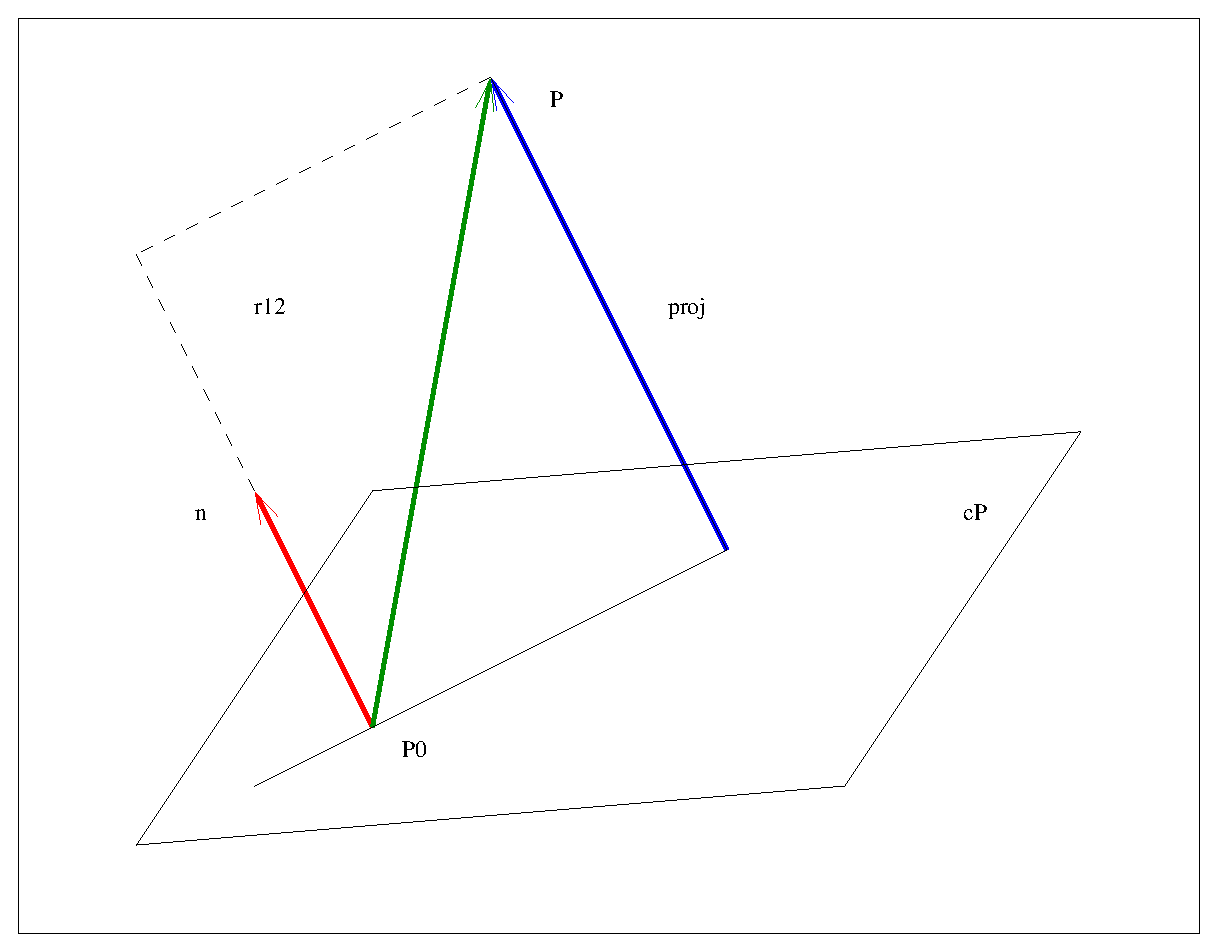
\includegraphics[height=2in]{../images/ok-distance_point_plane.eps}
    \end{figure}
    \end{columns}
\end{frame}

\begin{frame}
  \frametitle{Parallel lines}
    Lines
    $$L_1: \quad \textbf{r}= \textbf{r}_1+t\textbf{u}_1 \qquad L_2: \quad \textbf{r}= \textbf{r}_2+s\textbf{u}_2$$
\begin{columns}[t]
  \column[T]{6cm}
  \textcolor[rgb]{0.98,0.00,0.00}{Parallel} lines\\
    %\medskip
    \uncover<2->{
    $L_1 || L_2$ $\Longleftrightarrow$
    $\textbf{u}_1$, $\textbf{u}_2$ collinear $\Longleftrightarrow$
    $$\boxed{\textbf{u}_1 \times \textbf{u}_2 = \textbf{0}}$$}
    \uncover<3->{
    \textcolor[rgb]{0.98,0.00,0.00}{Distance}:
    $$d= d(L_1,L_2)  = d(P_1,L_2) = d(P_2,L_1)$$}
    \uncover<4->{
    $$d= d(L_1,L_2) = |\textbf{\text{orth}}_{\bm{u}_1} (\textbf{r}_2-\textbf{r}_1)|$$
    $$\boxed{d = \frac{|(\textbf{r}_2-\textbf{r}_1) \times \textbf{u}_1|}{|\textbf{u}_1|} =\frac{|(\textbf{r}_2-\textbf{r}_1) \times \textbf{u}_2|}{|\textbf{u}_2|}}$$}
    %\textcolor[rgb]{0.98,0.00,0.00}{Identical} lines: $d(L_1,L_2)=0$
    %$$\textbf{u}_1\times \textbf{u}_2 = \textbf{0} \text{ and }
    %(\textbf{r}_2-\textbf{r}_1) \times \textbf{u}_1 = \textbf{0}$$
  \column{6.5cm}
  \begin{figure}
        \psfrag{L1}{$L_1$}
        \psfrag{L2}{$L_2$}
        \psfrag{P1}{$P_1$}
        \psfrag{P2}{$P_2$}
        \psfrag{r21}{$\textbf{r}_2-\textbf{r}_1$}
        \psfrag{u1}{$\textbf{u}_1$}
        \psfrag{u2}{$\textbf{u}_2$}
        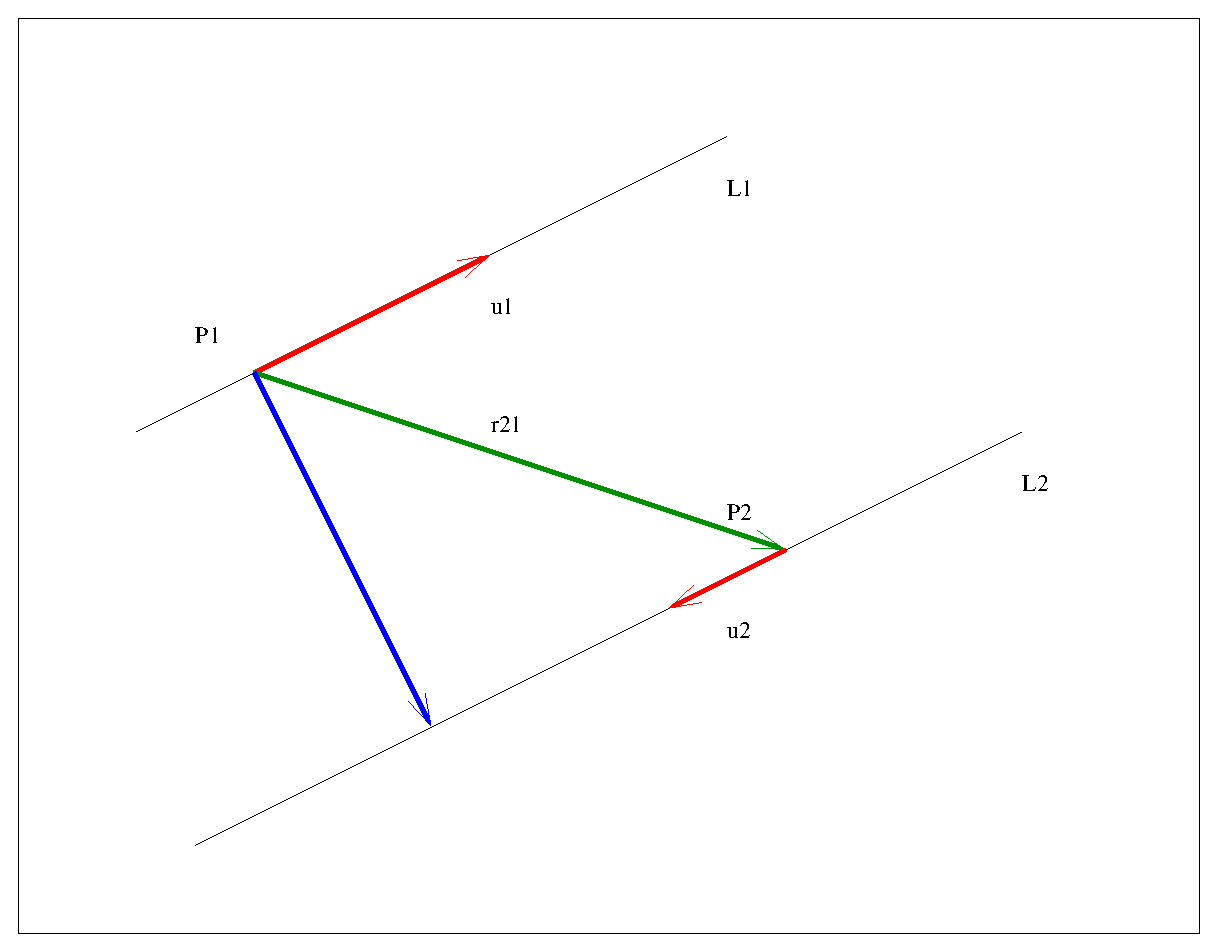
\includegraphics[height=2in]{../images/ok-distance_parallel_lines.eps}
    \end{figure}
\end{columns}

\end{frame}

\begin{frame}
\frametitle{Angle between lines}
Lines
    $$L_1: \quad \textbf{r}= \textbf{r}_1+t\textbf{u}_1 \qquad L_2: \quad \textbf{r}= \textbf{r}_2+s\textbf{u}_2$$

  \begin{columns}[t]
    \column[T]{6cm}
    \textcolor[rgb]{0.98,0.00,0.00}{Perpendicular} lines\\
    \uncover<2->{
    $L_1 \bot L_2$ $\Longleftrightarrow$
    $\textbf{u}_1 \bot \textbf{u}_2$ $\Longleftrightarrow$ \\
    $$\boxed{\textbf{u}_1 \cdot \textbf{u}_2 = 0}$$}
    %
    \uncover<3->{
    \textcolor[rgb]{0.98,0.00,0.00}{Angle} between lines\\}
    \uncover<4->{
        $\alpha$: angle between $L_1$, $L_2$ $\Longleftrightarrow$ \\
    $\alpha$: acute angle $\textbf{u}_1$, $\textbf{u}_2$}
    \uncover<5->{$\Longleftrightarrow$
    $$\boxed{\alpha = \arccos\left( \frac{|\textbf{u}_1 \cdot \textbf{u}_2|}{|\textbf{u}_1| \, |\textbf{u}_2|}\right) }$$}
    \column{6.5cm}
    \begin{figure}
        \psfrag{L1}{$L_1$}
        \psfrag{L2}{$L_2$}
        \psfrag{P1}{$P_1$}
        \psfrag{P2}{$P_2$}
        \psfrag{u1}{$\textbf{u}_1$}
        \psfrag{u2}{$\textbf{u}_2$}
        \psfrag{a}{$\alpha$}
        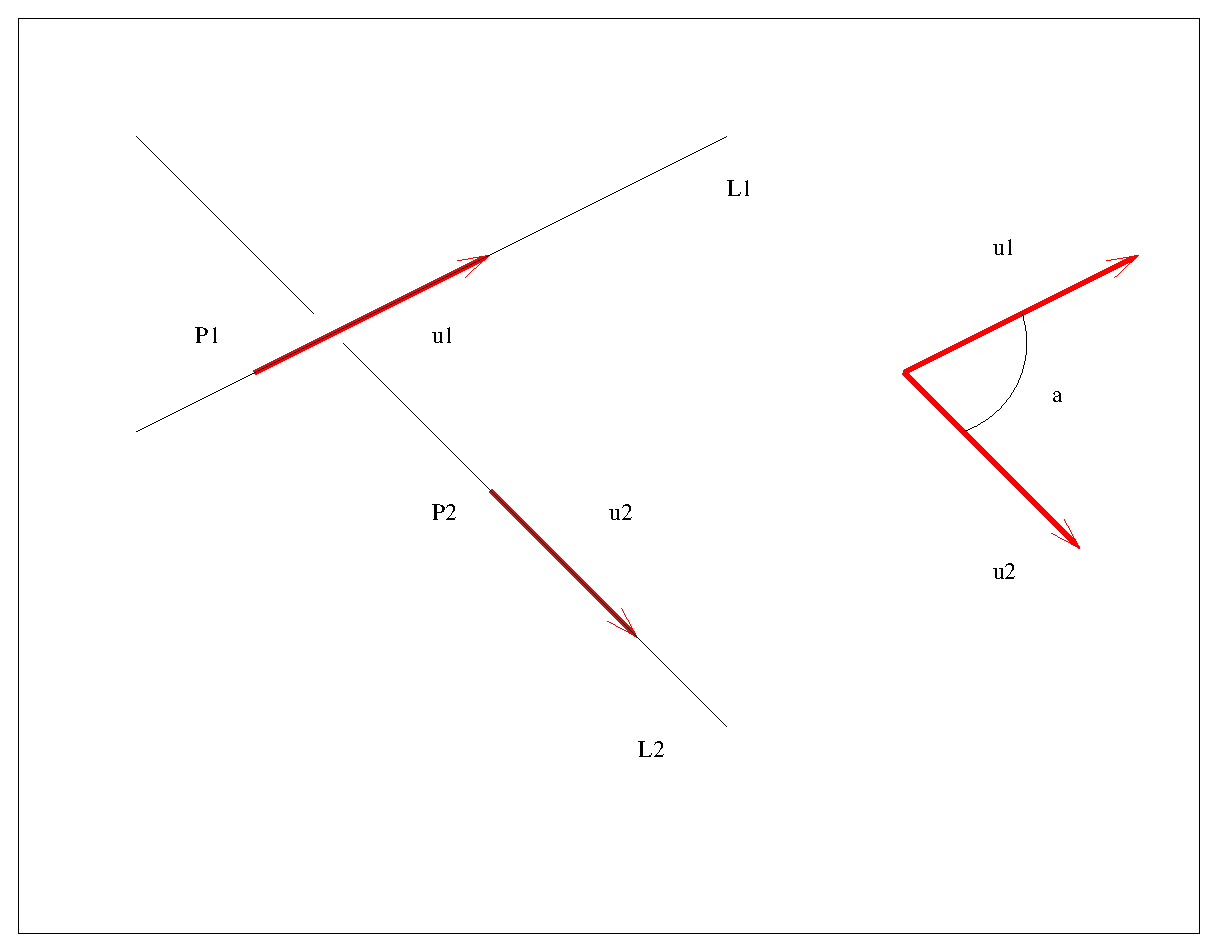
\includegraphics[height=2in]{../images/ok-angle_line_line.eps}
    \end{figure}
    %
  \end{columns}
\end{frame}

\begin{frame}
  \frametitle{Distance between lines}
     Lines
    $$L_1: \quad \textbf{r}= \textbf{r}_1+t\textbf{u}_1 \qquad L_2: \quad \textbf{r}= \textbf{r}_2+s\textbf{u}_2$$

   \begin{columns}[t]
    \column[T]{6cm}
    \textcolor[rgb]{0.98,0.00,0.00}{Skew lines}
    $$\textbf{n} = \textbf{u}_1 \times \textbf{u}_2 \neq \textbf{0}$$
    \textcolor[rgb]{0.98,0.00,0.00}{Distance}:
    $$
      d(L_1,L_2)  = |\textbf{\text{proj}}_{\bm{n}} (\textbf{r}_2-\textbf{r}_1)| =$$
      $$= \boxed{\frac{|(\textbf{r}_2-\textbf{r}_1)\cdot \textbf{n}|}{|\textbf{n}|}}=
      \frac{|(\textbf{r}_2-\textbf{r}_1)\cdot (\textbf{u}_1\times \textbf{u}_2)|}{|\textbf{u}_1\times \textbf{u}_2|}$$
    \textcolor[rgb]{0.98,0.00,0.00}{Intersecting} lines: $d(L_1,L_2)=0$
    $$\textbf{u}_1\times \textbf{u}_2 \neq \textbf{0}$$
    $$(\textbf{r}_2-\textbf{r}_1) \cdot (\textbf{u}_1\times \textbf{u}_2) = 0$$

    \column{6.5cm}
    \only<1>{\begin{figure}
        \psfrag{L1}{$L_1$}
        \psfrag{L2}{$L_2$}
        \psfrag{P1}{$P_1$}
        \psfrag{P2}{$P_2$}
        \psfrag{n}{$\textbf{n}$}
        \psfrag{r21}{$\textbf{r}_2-\textbf{r}_1$}
        \psfrag{u1}{$\textbf{u}_1$}
        \psfrag{u2}{$\textbf{u}_2$}
        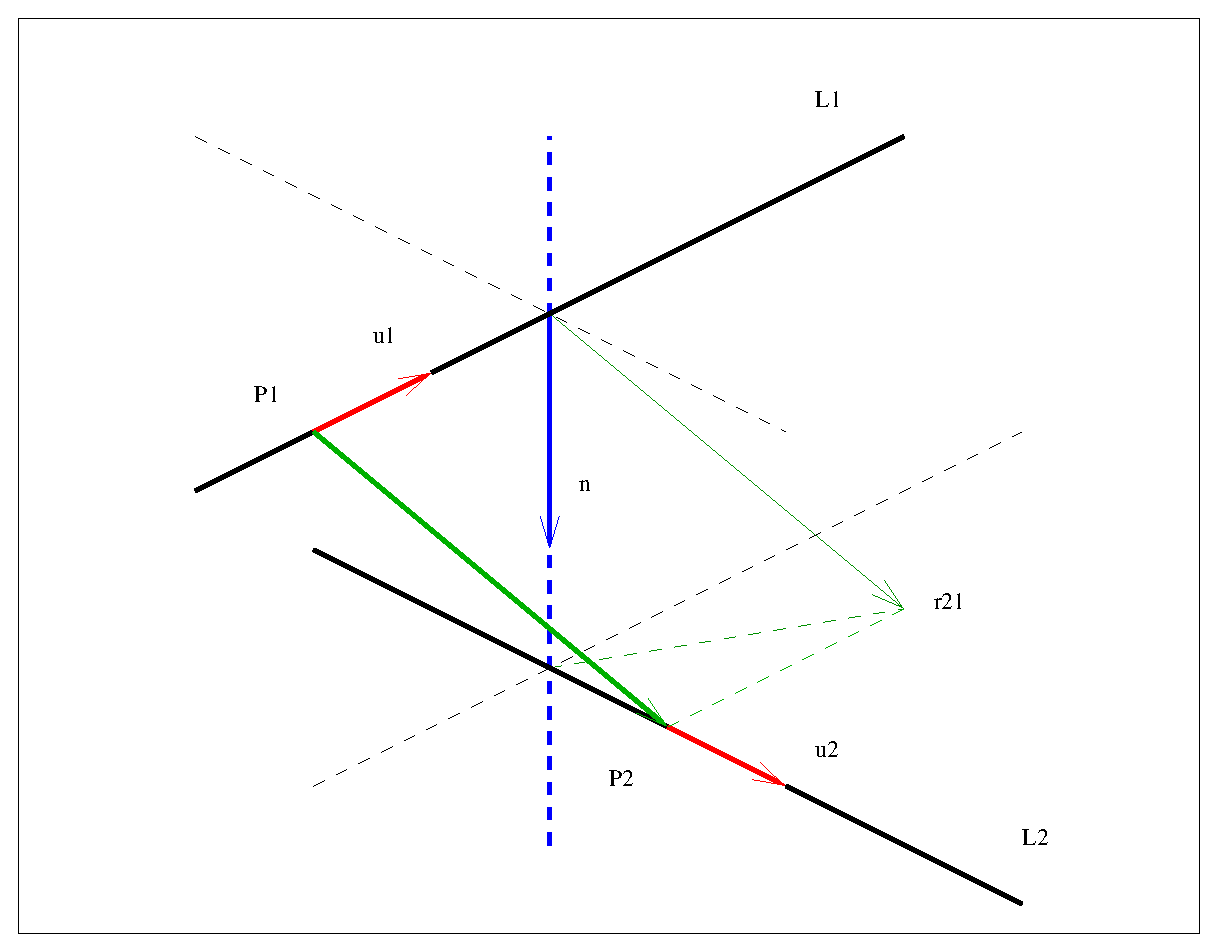
\includegraphics[height=2in]{../images/ok-distance_skew_lines.eps}
    \end{figure}}
    \only<2>{\begin{figure}
        \psfrag{L1}{$L_1$}
        \psfrag{L2}{$L_2$}
        \psfrag{P1}{$P_1$}
        \psfrag{P2}{$P_2$}
        \psfrag{n}{$\textbf{n}$}
        \psfrag{r21}{$\textbf{r}_2\!-\!\textbf{r}_1$}
        \psfrag{u1}{$\textbf{u}_1$}
        \psfrag{u2}{$\textbf{u}_2$}
        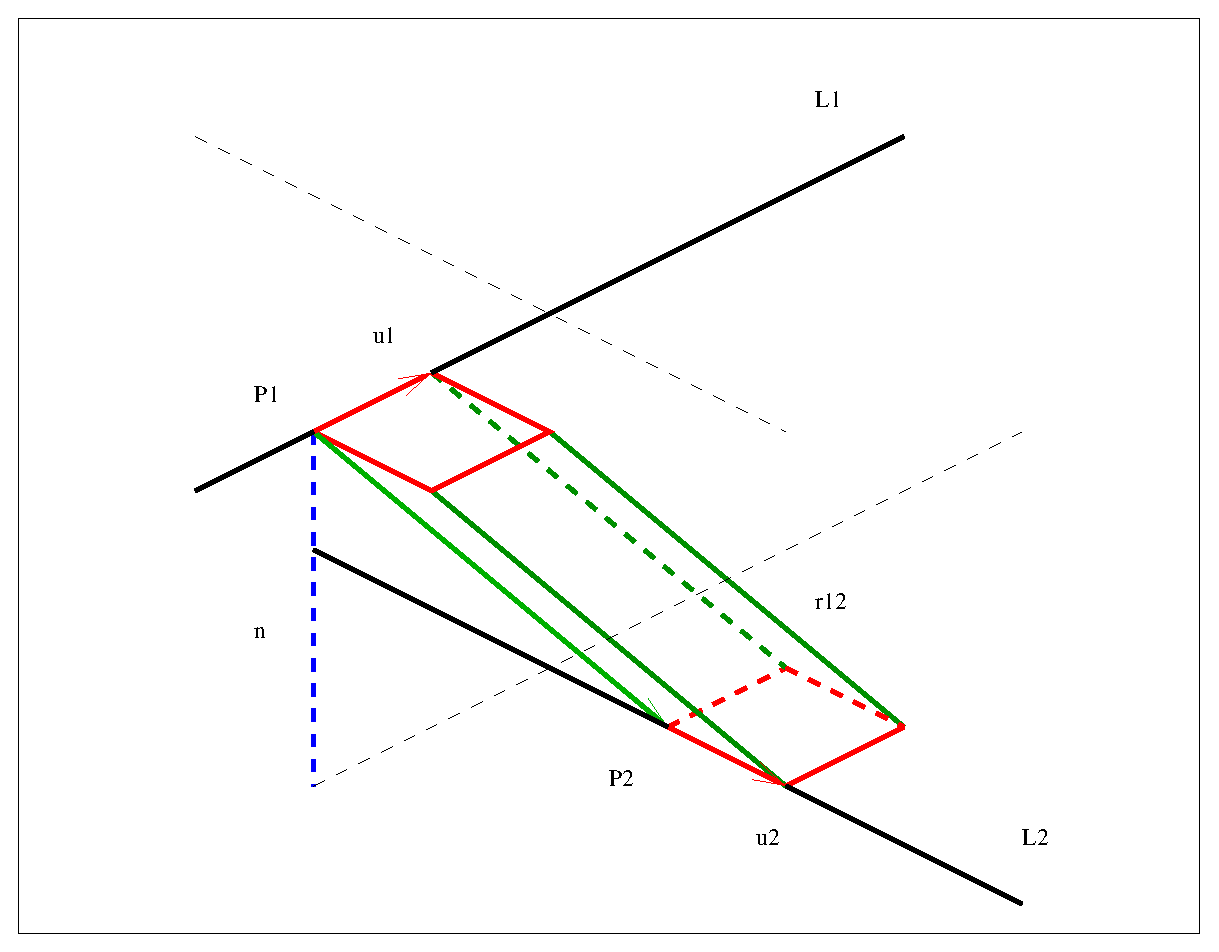
\includegraphics[height=2in]{../images/ok-distance_skew_lines_box.eps}
    \end{figure}
    }
  \end{columns}
\end{frame}



\begin{frame}
  \frametitle{Parallel line and plane}
     Line $L: \quad \textbf{r}= \textbf{r}_1+t\textbf{u}$\hspace{2cm}
     Plane $\mathcal{P}: \quad (\textbf{r}-\textbf{r}_0) \cdot \textbf{n} = 0$
\bigskip
  \begin{columns}[t]
    \column{6cm}
    Line \textcolor[rgb]{0.98,0.00,0.00}{parallel} to plane\\
    \uncover<2->{
    $L || \mathcal{P}$ $\Longleftrightarrow$
    $\textbf{u} \bot \textbf{n}$ $\Longleftrightarrow$
    $$\boxed{\textbf{u} \cdot \textbf{n} = 0}$$}
    \uncover<3->{
    \textcolor[rgb]{0.98,0.00,0.00}{Distance} from $L$ to $\mathcal{P}$:
    $$d(L,\mathcal{P}) = d(P_1,\mathcal{P})$$}
    \uncover<4->{
    $$d=|\textbf{\text{orth}}_{\bm{u}}(\textbf{r}_1-\textbf{r}_0)| =
    |\textbf{\text{proj}}_{\bm{n}} (\textbf{r}_1-\textbf{r}_0)|$$
    $$d = \frac{|(\textbf{r}_1-\textbf{r}_0) \times \textbf{u}|}{|\textbf{u}|} =
    \textcolor[rgb]{0.98,0.00,0.00}{\frac{|(\textbf{r}_1-\textbf{r}_0)\cdot \textbf{n}|}{|\textbf{n}|}}$$}
    \column{6.5cm}
    \begin{figure}
        \psfrag{L}{$L$}
        \psfrag{cP}{$\mathcal{P}$}
        \psfrag{P1}{$P_1(\textbf{r}_1)$}
        \psfrag{P0}{$P_0(\textbf{r}_0)$}
        \psfrag{u}{$\textbf{u}$}
        \psfrag{n}{$\textbf{n}$}
        \psfrag{r01}{$\textbf{r}_1-\textbf{r}_0$}
        \psfrag{proj}{$\textbf{\text{proj}}_{\bm{n}} (\textbf{r}_1\!-\!\textbf{r}_0)$}
        \psfrag{orth}{$\textbf{\text{orth}}_{\bm{u}}(\textbf{r}_1\!-\!\textbf{r}_0)$}
        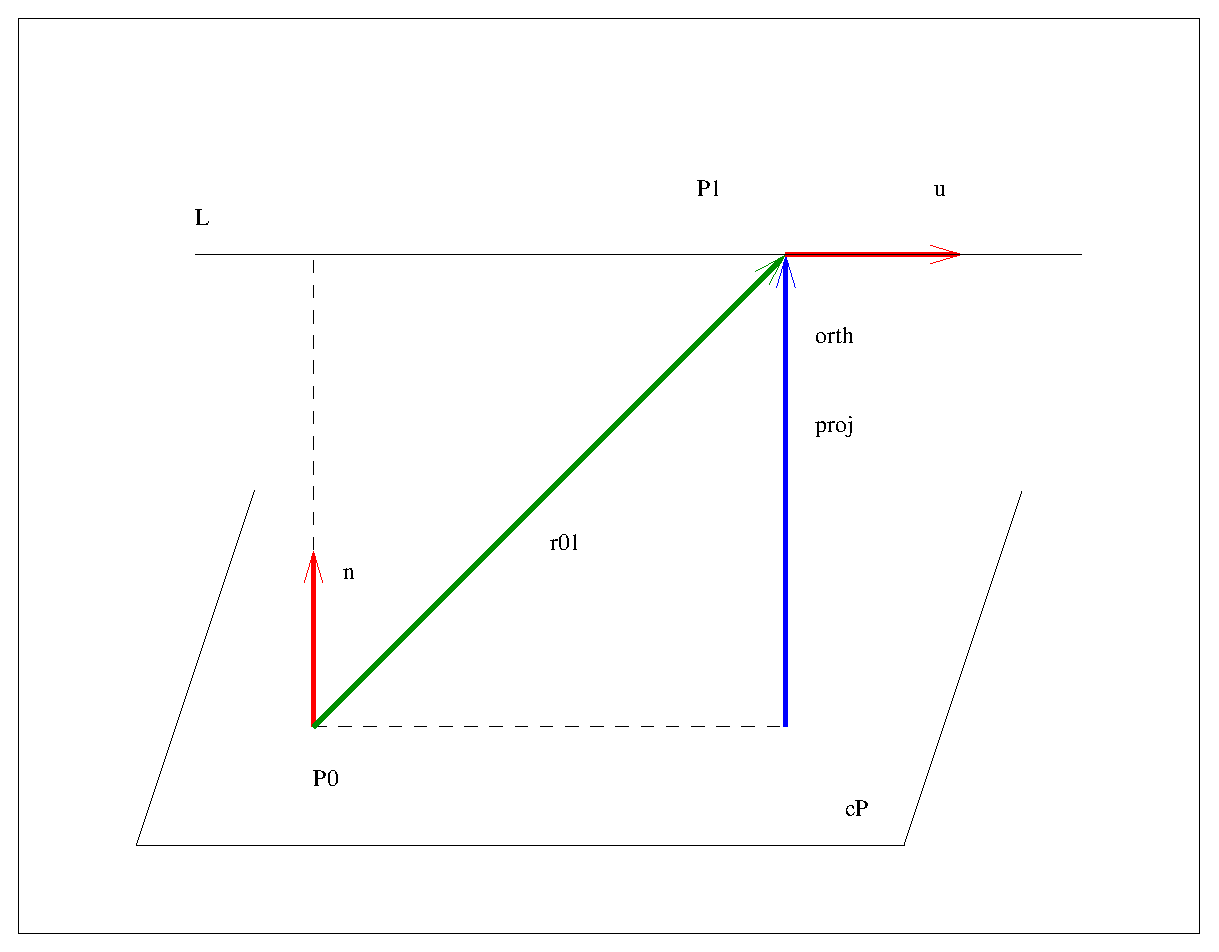
\includegraphics[height=2in]{../images/ok-parallel_line_plane.eps}
    \end{figure}
    %
  \end{columns}
\end{frame}


\begin{frame}
  \frametitle{Angle between line and plane}
     Line $L: \quad \textbf{r}= \textbf{r}_1+t\textbf{u}$ \hspace{2cm}
     Plane $\mathcal{P}: \quad (\textbf{r}-\textbf{r}_0) \cdot \textbf{n} = 0$

   \begin{columns}[t]
    \column[T]{6cm}
    %
    Line \textcolor[rgb]{0.98,0.00,0.00}{perpendicular} to plane\\
    \uncover<2->{
    $L \bot \mathcal{P}$ $\Longleftrightarrow$
    $\textbf{u} \| \textbf{n}$ $\Longleftrightarrow$ \\
    $$\boxed{\textbf{u} \times \textbf{n} = \textbf{0}}$$}
    %
    \uncover<3->{
    \textcolor[rgb]{0.98,0.00,0.00}{Angle} between line and plane\\
    %
    $\alpha$: angle between $L$, $\mathcal{P}$ $\Longleftrightarrow$ \\
    $\alpha$: acute angle $\textbf{u}$, $\textbf{\text{orth}}_{\bm{n}}\textbf{u}$} \uncover<4->{$\Longleftrightarrow$
    $$\boxed{\alpha = \arcsin\left( \frac{|\textbf{u} \cdot \textbf{n}|}{|\textbf{u}| \, |\textbf{n}|}\right) }$$}
    \uncover<5->{\textcolor[rgb]{0.98,0.00,0.00}{Intersection}:}
    \uncover<6->{$$(\textbf{r}_1+t\textbf{u}-\textbf{r}_0) \cdot \textbf{n} = 0$$
    $$(\textbf{r}_1-\textbf{r}_0)\cdot \textbf{n} + t \textbf{u} \cdot \textbf{n} = 0$$
    Solve for $t$.}
    \column{6.5cm}
    %
    \begin{figure}
        \psfrag{L}{$L$}
        \psfrag{cP}{$\mathcal{P}$}
        \psfrag{P0}{$P_0(\textbf{r}_0)$}
        \psfrag{P1}{$P_1(\textbf{r}_1)$}
        \psfrag{P2}{$P_2$}
        \psfrag{a}{$\alpha$}
        \psfrag{orth}{$\textbf{\text{orth}}_{\bm{n}}\textbf{u}$}
        \psfrag{u}{$\textbf{u}$}
        \psfrag{n}{$\textbf{n}$}
        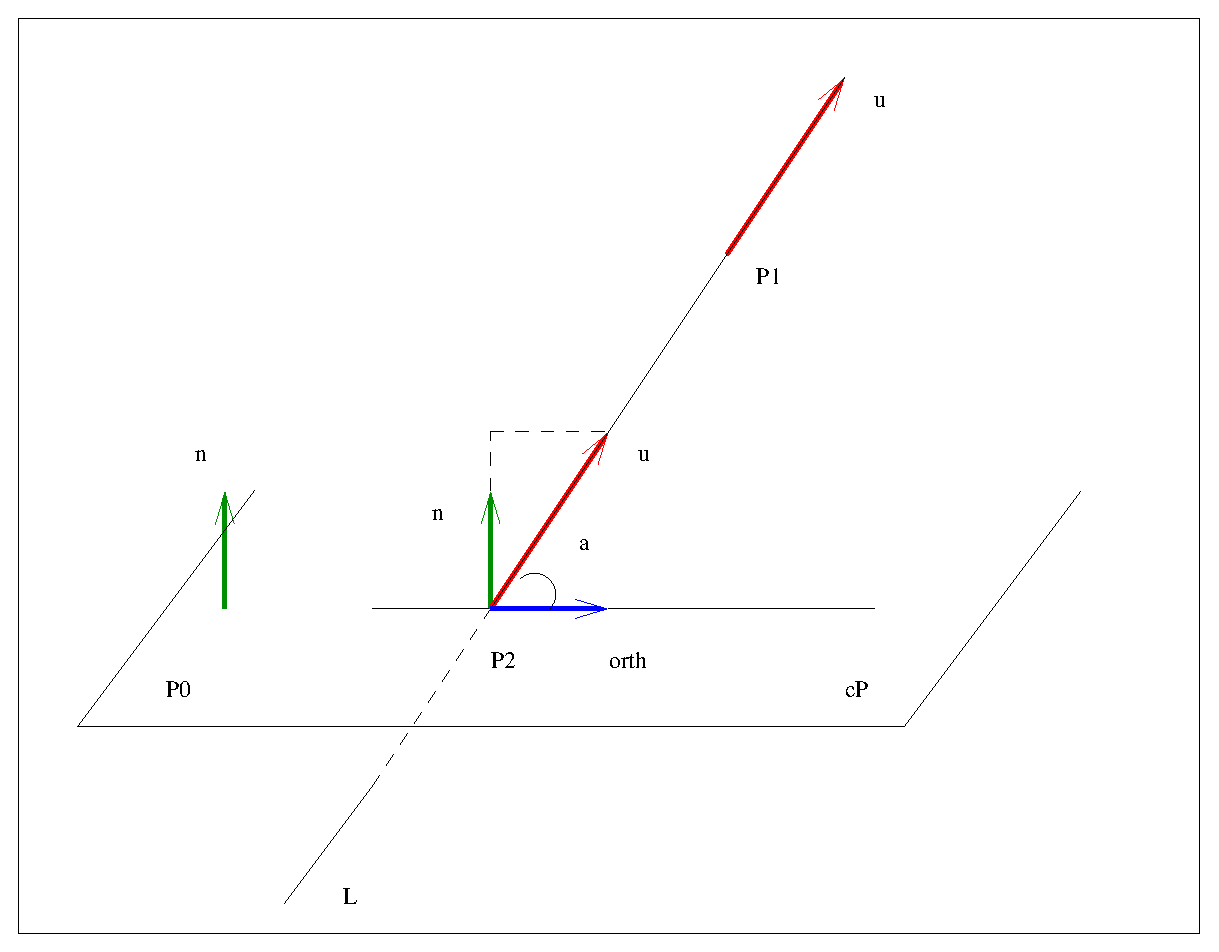
\includegraphics[height=2in]{../images/ok-angle_line_plane.eps}
    \end{figure}
  \end{columns}
\end{frame}

\begin{frame}
  \frametitle{Parallel planes}
     Planes
     $\mathcal{P}_1: \quad (\textbf{r} - \textbf{r}_1) \cdot \textbf{n}_1 = 0$
     \hspace{2cm}
     $\mathcal{P}_2: \quad (\textbf{r} - \textbf{r}_2) \cdot \textbf{n}_2 = 0$

  \begin{columns}[t]
    \column[T]{6cm}
    \textcolor[rgb]{0.98,0.00,0.00}{Parallel} planes:  \\
    \uncover<2->{$\mathcal{P}_1 || \mathcal{P}_2$ $\Longleftrightarrow$ $\textbf{n}_1$, $\textbf{n}_2$ collinear $\Longleftrightarrow$
    $$\boxed{\textbf{n}_1 \times \textbf{n}_2 = \textbf{0}}$$}
    \uncover<3->{
    \textcolor[rgb]{0.98,0.00,0.00}{Distance} between parallel planes:
    $$d(\mathcal{P}_1,\mathcal{P}_2) =
    |\textbf{\text{proj}}_{\textbf{n}_1} (\textbf{r}_2-\textbf{r}_1)| = $$
    $$=\boxed{\frac{|(\textbf{r}_2-\textbf{r}_1)\cdot \textbf{n}_1|}{|\textbf{n}_1|}}$$}
    \uncover<4->{\textcolor[rgb]{0.98,0.00,0.00}{Scalar} equations:\\
    $\mathcal{P}_1 : \quad ax+by+cz = d_1$\\
    $\mathcal{P}_2 : \quad ax+by+cz = d_2$
    $$\boxed{d(\mathcal{P}_1,\mathcal{P}_2) = \frac{|d_2-d_1|}{\sqrt{a^2+b^2+c^2}}}$$}
    \column[T]{6.5cm}
    \begin{figure}
        \psfrag{cP1}{$\mathcal{P}_1$}
        \psfrag{cP2}{$\mathcal{P}_2$}
        \psfrag{P1}{$P_1(\textbf{r}_1)$}
        \psfrag{P2}{$P_2(\textbf{r}_2)$}
        \psfrag{n1}{$\textbf{n}_1$}
        \psfrag{n2}{$\textbf{n}_2$}
        \psfrag{r12}{$\textbf{r}_2\!-\!\textbf{r}_1$}
        \psfrag{proj}{$\textbf{\text{proj}}_{\bm{n}_1} (\textbf{r}_1\!-\!\textbf{r}_0)$}
        \includegraphics[height=2in]{../images/ok-parallel_plane_plane.eps}
    \end{figure}
    %
  \end{columns}
\end{frame}

\begin{frame}
  \frametitle{Angle between planes}
     Planes
     $\mathcal{P}_1: \quad (\textbf{r} - \textbf{r}_1) \cdot \textbf{n}_1 = 0$
     \hspace{2cm}
     $\mathcal{P}_2: \quad (\textbf{r} - \textbf{r}_2) \cdot \textbf{n}_2 = 0$

  \begin{columns}[t]
    \column[T]{6cm}
    \textcolor[rgb]{0.98,0.00,0.00}{Angle} $\alpha$ between planes:
    \uncover<2->{$$\alpha = \text{acute angle} (\textbf{n}_1,\textbf{n}_2) $$
    $$\alpha =
    \arccos{\left( \frac{|\textbf{n}_1 \cdot \textbf{n}_2|}{|\textbf{n}_1|\, |\textbf{n}_2|}\right)}$$}
    \uncover<3->{\textcolor[rgb]{0.98,0.00,0.00}{Perpendicular} planes:}
    \uncover<4->{$$\alpha = \frac{\pi}{2} \Longleftrightarrow \boxed{\textbf{n}_1 \cdot \textbf{n}_2 = 0}$$}
    \uncover<5->{Direction of \textcolor[rgb]{0.98,0.00,0.00}{line of intersection}:}
    \uncover<6->{$$\textbf{u} = \textbf{n}_1 \times \textbf{n}_2$$}
    \column[T]{6.5cm}
    \begin{figure}
        \psfrag{cP1}{$\mathcal{P}_2$}
        \psfrag{cP2}{$\mathcal{P}_1$}
        \psfrag{P1}{$P_2$}
        \psfrag{P2}{$P_1$}
        \psfrag{n1}{$\textbf{n}_2$}
        \psfrag{n2}{$\textbf{n}_1$}
        \psfrag{a}{$\alpha$}
        \psfrag{u}{$\textbf{u}$}
        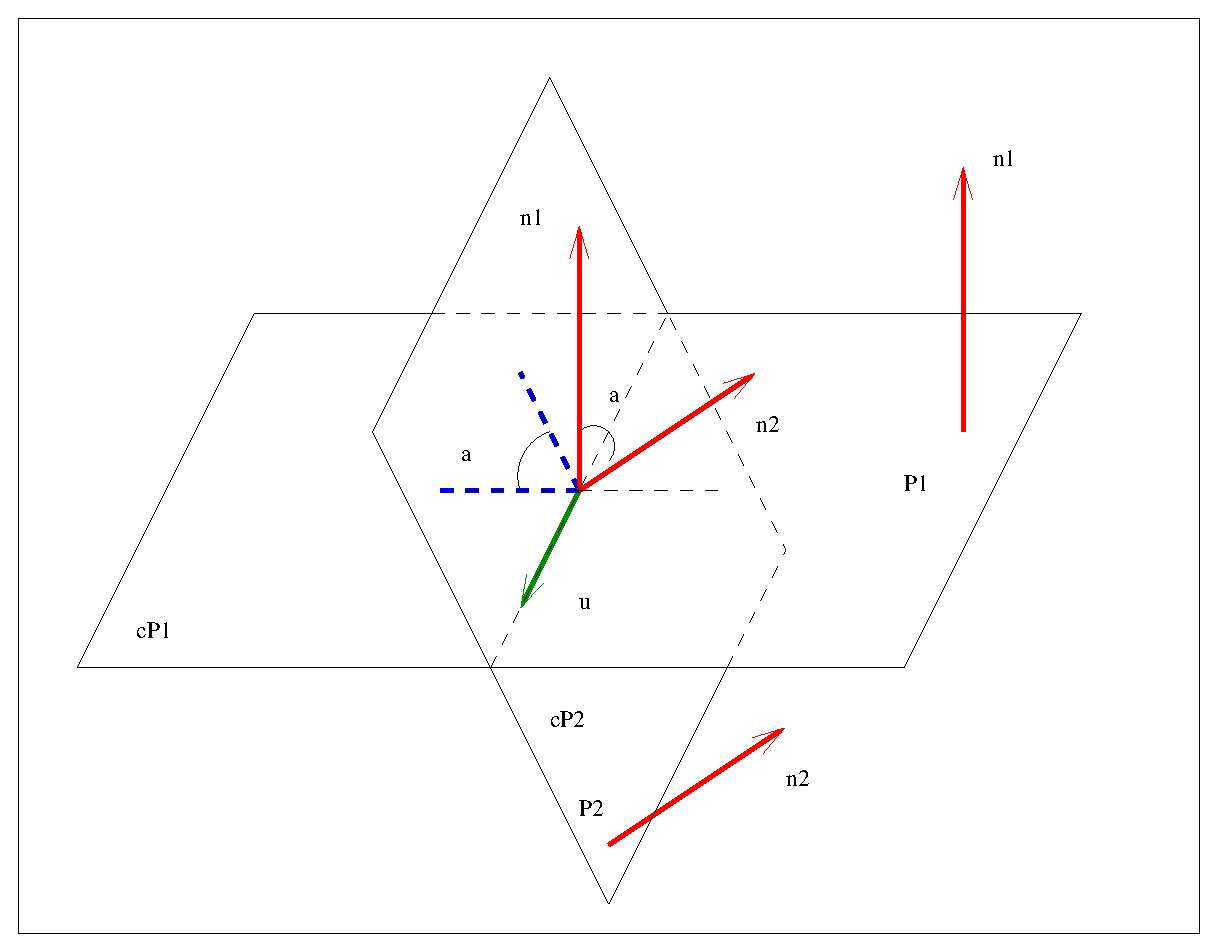
\includegraphics[height=2in]{../images/ok-angle_plane_plane.eps}
    \end{figure}
    %
  \end{columns}
\end{frame}
